\documentclass{article}
\usepackage{amsmath}
\usepackage{graphicx}
\usepackage{hyperref}
\usepackage{algorithm}
\usepackage{algpseudocode}
\title{IPF}
\author{Max Lang}
\date{January 2024}


\begin{document}

\maketitle

\section{Definition of the Algorithm}

The Iterative Proportional Fitting (IPF) algorithm is a statistical procedure used to adjust the values in a multi-way table such that the marginal totals match specified targets. The algorithm starts with an initial distribution (often uniform) and iteratively scales the distribution across different dimensions (or margins) to match the known marginal distributions.

$$
\begin{aligned}
p^{(t+1)}\left(x_V\right) & =p^{(t)}\left(x_V\right) \cdot \frac{\hat{p}\left(x_C\right)}{p^{(t)}\left(x_C\right)} \\
& =p^{(t)}\left(x_{V \backslash C} \mid x_C\right) \cdot \hat{p}\left(x_C\right) .
\end{aligned}
$$

\begin{algorithm}
\caption{Iterative Proportional Fitting (IPF) algorithm}
\begin{algorithmic}[1]
\Function{IPF}{collection of consistent margins $q(x_{C_i})$ for sets $C_1, \ldots, C_k$}
    \State set $p(x_V)$ to uniform distribution;
    \While{max$_i$ max$_{x_{C_i}} \left| p(x_{C_i}) - q(x_{C_i}) \right| > \text{tol}$}
        \For{$i \in 1, \ldots, k$}
            \State update $p(x_V)$ to $p(x_V | x_{C_i}) \cdot q(x_{C_i});$
        \EndFor
    \EndWhile
    \State \Return distribution $p$ with margins $p(x_{C_i}) = q(x_{C_i})$.
\EndFunction
\end{algorithmic}
\end{algorithm}

\begin{itemize}
    \item IPF converges to the MLE $\hat{p}\left(x_V\right)$
    \item Note that the update ensures that the moments for the sufficient statistics involving the clique $C$ are matched
    \item After each update step the joint distribution remains Markov with respect to $\mathcal{G}$ : this can be seen easily by considering the factorization
    \item Performing each step increases the likelihood, and since the log-likelihood is strictly concave, this sort of co-ordinate based iterative updating scheme will converge to the global maximum.
\end{itemize}



\section{Intuition and Explanation of the Algorithm Idea}

Intuitively, IPF operates like a sculptor refining a block of stone. It begins with a rough shape (the initial distribution) and iteratively chips away discrepancies between the observed and expected marginal distributions. Each iteration adjusts the "stone" to better fit the "outline" provided by the marginals. The "chiseling" happens one dimension at a time, proportionally adjusting the values so that the totals along that dimension match the known marginals, while keeping the ratios within the distribution consistent.

\section{Example}

\subsection{2D IPF}

Consider a \(2 \times 2\) table with two binary variables, \(X\) and \(Y\), with initial counts set uniformly. Suppose we have marginal totals for \(X\) and \(Y\) from external sources. IPF will adjust the counts in the table so that the totals for \(X\) and \(Y\) match the provided marginals. If \(X_1\) should total to 10 and \(X_0\) to 90, and similarly for \(Y\), the algorithm will scale the rows and columns iteratively to match these totals.


\subsubsection{Example}
Consider the 4-cycle in the figure, with cliques $\{1, 2 \} , \{ 2, 3 \} , \{ 3, 4 \} , \{ 1, 4 \}$ .

Suppose we have data from $n = 96$ observations as shown in the table below (the column ‘count’).


\begin{figure}
    \centering
    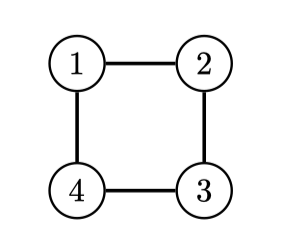
\includegraphics[width=0.5\linewidth]{overviews/graphical-models/figures/Graph.png}
\end{figure}

\begin{figure}
    \centering
    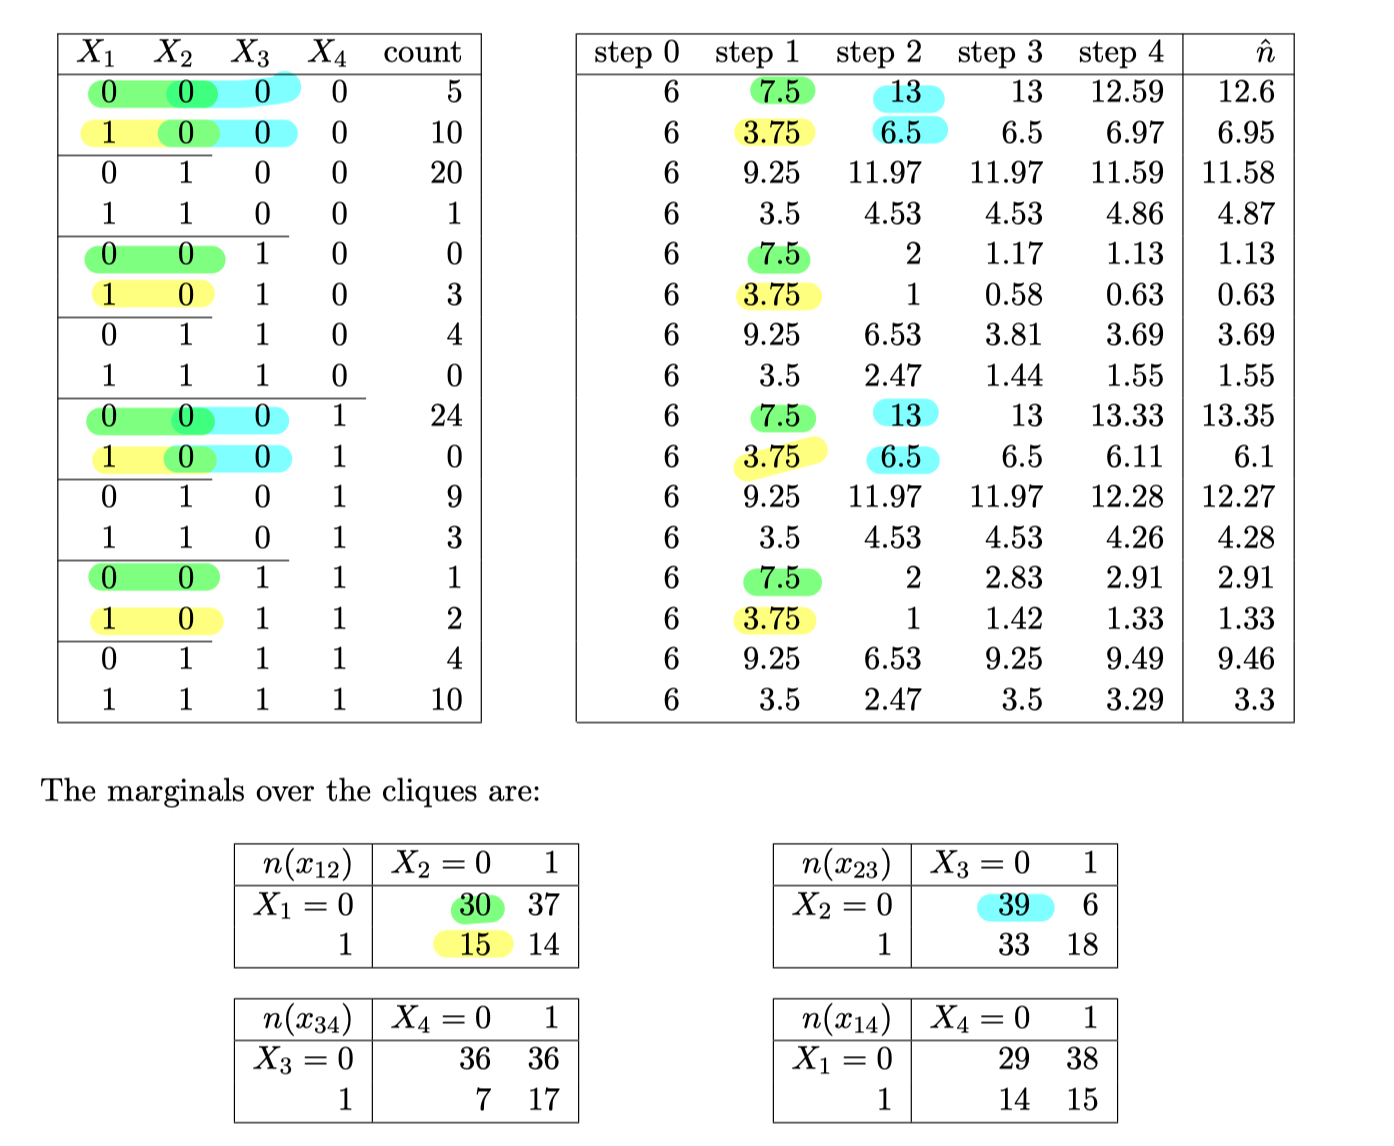
\includegraphics[width=0.8\linewidth]{overviews/graphical-models/figures/IPF_Tables.png}
\end{figure}

To implement IPF, we start with a uniform table, given in the column `step 0'. We then scale the entries so as to match the \(X_1, X_2\) margin above. For instance, the four entries corresponding to \(X_1 = X_2 = 0\) are scaled to add up to 30; this gives the column `step 1'. This is repeated for each of the other cliques, giving steps 2--4. By the fourth step the distribution of all cliques has been updated, but note that the margin over \(X_1, X_2\) is now 29.96, 15.04, 37.04, 13.96. We keep cycling until the process converges to the final column, which matches all four margins.


\subsection{3D IPF}

For a 3D table (imagine a Rubik's cube of data), say with variables \(X\), \(Y\), \(Z\), the IPF would adjust the \(2D\) "faces" of the cube to match the \(2D\) marginals, and then \(1D\) "edges" to match the \(1D\) marginals, continually cycling through dimensions until the entire cube's marginal distributions match the specified targets.

\begin{figure}
    \centering
    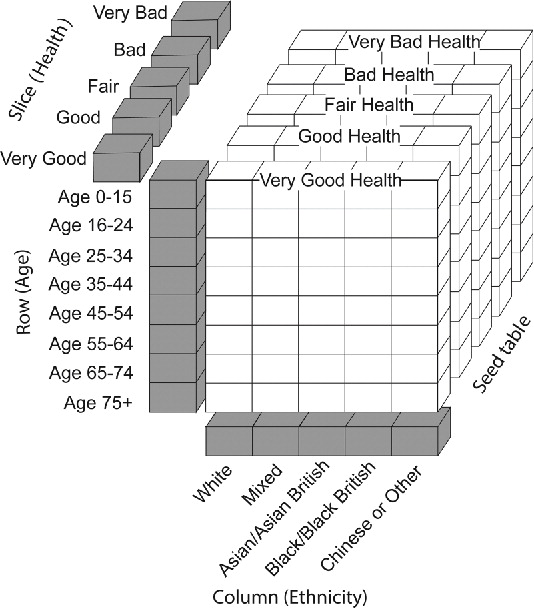
\includegraphics[width=0.75\linewidth]{overviews/graphical-models/figures/rtpg_a_1099449_f0002_b.jpg}
    \caption{Iterative proportional fitting over three dimensions (age, ethnicity, and health)}
    \label{fig:enter-label}
\end{figure}

\section{Why is it Useful in Terms of Graphical Models?}

In graphical models, especially those dealing with categorical data, IPF is invaluable because it allows us to estimate joint distributions from partial or incomplete data. Given a set of variables with known dependencies (the graph structure), we can use IPF to "fill in" the joint distribution by ensuring consistency with observed marginals. This is particularly useful in cases where the full joint distribution is unknown or cannot be directly observed.

\section{Conclusion}

The IPF algorithm is a powerful tool for adjusting multi-dimensional tables to fit known marginal distributions. Its iterative nature allows for flexible adjustments across various dimensions, ensuring that the final distribution is consistent with known marginals. This is particularly useful in graphical models where the structure of the graph informs the dependencies between variables, and the IPF algorithm can leverage this structure to estimate the full joint distribution. By doing so, IPF facilitates the use of graphical models in statistical inference, prediction, and decision-making processes where understanding the joint behavior of multiple variables is crucial.

\end{document}

